\frame {\frametitle{ Data management }
    \begin{itemize}
	\item Victor remains interim PM until April 
	\item Have been trying to get an idea of DM organisation - talking to DMLT and TCAMS 
	\item Following are some observations and draft ideas 

    \end{itemize}

    {\bf   Look out for a  new version of LDM-294 - DM Management Plan}
    \begin{itemize}
	\item It will detail roles and responsibilities in DM
    \end{itemize}
}


\frame {\frametitle{ DM Organisation}

      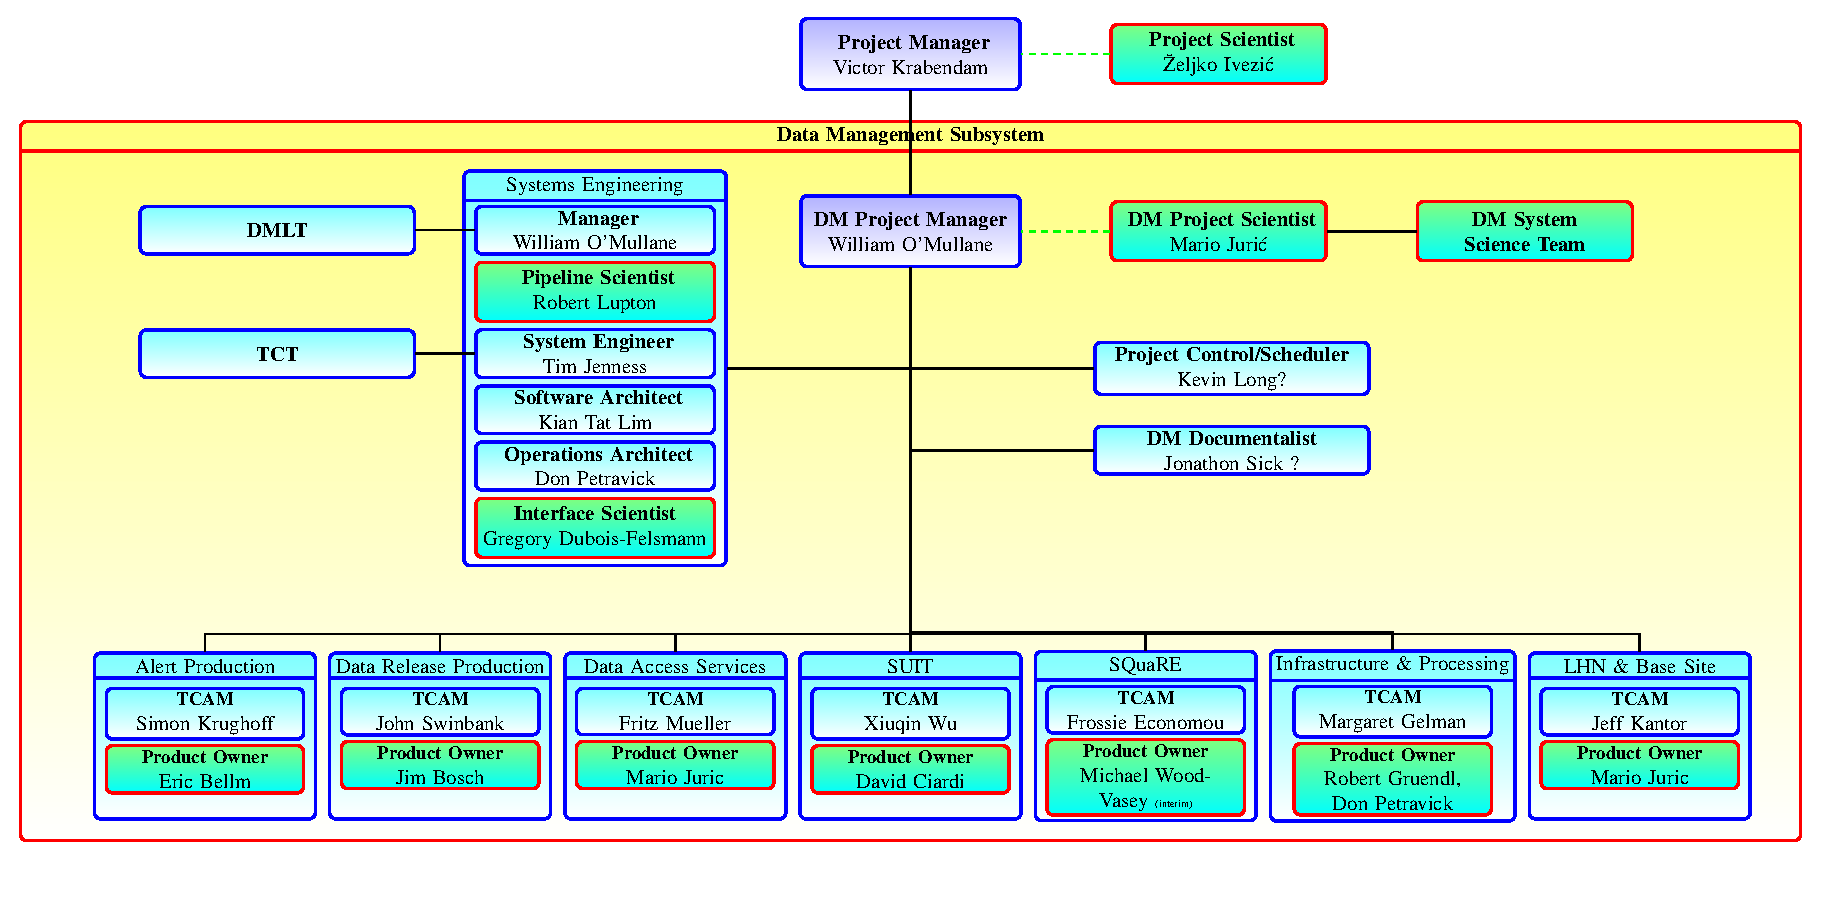
\includegraphics[width=1.0\textwidth]{images/DmOrg}\\
}

\frame {\frametitle{ DM architecture \& products}
	\begin{itemize}
	\item Would like to get  a list of products in DM
	\item Related to understanding the DM architecture - KT working on LDM-148 update more from him in a while
	\item Those are not Data Products - mostly Systems and Software artefacts
	\item For each product identify {\em Product Owner} and manager.
	\item This would change the org chart ..
	
	\end{itemize}

}

\frame {\frametitle{ Risk Management and other processes ..}
Also in LDM-294:
	\begin{itemize}
	 \item Would like an open Risk approach - anyone can raise a risk (Tim working on that)	
	 \item Document management - in next slid as
	 \item Configuration control 
	 \item Product assurance  and Scientific Validation 
	\item \ldots
	\end{itemize}
Mainly these will be high level and point to the details in other documents. 

}
